\documentclass[12pt,letterpaper]{article}
\textwidth 6.5in
\textheight 9.in
\oddsidemargin 0in
\headheight 0in
\usepackage{graphicx}
\usepackage{fancybox}
\usepackage[utf8]{inputenc}
\usepackage{epsfig,graphicx}
\usepackage{multicol,pst-plot}
\usepackage{pstricks}
\usepackage{amsmath}
\usepackage{amsfonts}
\usepackage{amssymb}
\usepackage{eucal}
\usepackage[left=2cm,right=2cm,top=2cm,bottom=2cm]{geometry}
\pagestyle{empty}
\DeclareMathOperator{\tr}{Tr}
\newcommand*{\op}[1]{\check{\mathbf#1}}
\newcommand{\bra}[1]{\langle #1 |}
\newcommand{\ket}[1]{| #1 \rangle}
\newcommand{\braket}[2]{\langle #1 | #2 \rangle}
\newcommand{\mean}[1]{\langle #1 \rangle}
\newcommand{\opvec}[1]{\check{\vec #1}}
\renewcommand{\sp}[1]{$${\begin{split}#1\end{split}}$$}



\usepackage{lipsum}
\usepackage{fancyhdr}
\usepackage{mdframed}
\usepackage{textpos}
\usepackage{tikz}
\usetikzlibrary{arrows.meta}
\tikzset{>={Latex[width=3mm,length=3mm]}}
\usepackage{hyperref}
\hypersetup{
    colorlinks=true,
    linkcolor=blue,
    urlcolor=blue,
    }
% \usepackage{showframe}


\usepackage{listings}
\usepackage{color}

\definecolor{codegreen}{rgb}{0,0.6,0}
\definecolor{codegray}{rgb}{0.5,0.5,0.5}
\definecolor{codepurple}{rgb}{0.58,0,0.82}
\definecolor{backcolour}{rgb}{0.95,0.95,0.92}

\lstdefinestyle{mystyle}{
	backgroundcolor=\color{backcolour},   
	commentstyle=\color{codegreen},
	keywordstyle=\color{magenta},
	numberstyle=\tiny\color{codegray},
	stringstyle=\color{codepurple},
	basicstyle=\footnotesize,
	breakatwhitespace=false,         
	breaklines=true,                 
	captionpos=b,                    
	keepspaces=true,                 
	numbers=left,                    
	numbersep=5pt,                  
	showspaces=false,                
	showstringspaces=false,
	showtabs=false,                  
	tabsize=2
}

\lstset{style=mystyle}
\fancypagestyle{frontPage}{\fancyhf{}\renewcommand{\headrulewidth}{0pt}
\fancyfoot[C]{1-\thepage}
\fancyfoot[R]{UCSD}}


\begin{document}
\thispagestyle{frontPage}
\pagestyle{fancy}
\fancyhead{}
\fancyhead[L]{\textbf{DSC190 - Network Science and Graph Theory}}
\fancyhead[R]{\textbf{UCSD - Fall 2022}}
\fancyfoot{}
\fancyfoot[C]{1-\thepage}
\fancyfoot[R]{UCSD}
\renewcommand{\footrulewidth}{0.4pt}% default is 0pt

 

\begin{mdframed}[linewidth=1pt, innerleftmargin=3cm, innerrightmargin=1cm]
\begin{textblock*}{\textwidth}(-2.9cm,0cm)
\textbf{DSC190: Network Science and Graph Theory}
\end{textblock*}

\begin{textblock*}{\textwidth}(11.95cm,0cm)
\textbf{Fall 2022}
\end{textblock*}
\vspace{1cm}

\begin{textblock*}{\textwidth}(1.5cm,0cm)
\text{\LARGE{Homework Assignment 1}}
\end{textblock*}

\vspace{0.3cm}
\begin{textblock*}{\textwidth}(-1cm,0.5cm)
\centering\small{\textbf{Topics:} (Matrix Formalism, Graph Representation, Network Metrics, Erdős-Rényi Networks, Snobbish Networks)}
\end{textblock*}

\vspace{1.8cm}
\begin{textblock*}{\textwidth}(1.8cm,-2.3cm)
\hspace{10cm}
\includegraphics[height=2cm]{ucsd.png}
\end{textblock*}

\vspace{1.4cm}
\begin{textblock*}{\textwidth}(2.1cm,-1.2cm)
\hspace{-0.6cm}\small{Instructor: \textbf{Prof. Gal Mishne}} \newline
\small{Deadline: \textbf{Wednesday Oct. 12 (10/12/2022)}} \newline
\small{Submission: \textbf{Gradescope}}
\end{textblock*}
\end{mdframed}

%%%%%%%%%%%%%%%%%%%%%%%%%%%%%%%%%%%%%%%%%%%%%%%%%%%%%%%%%%%%%%%%%%%%%%%%

\bigskip
\bigskip

\begin{enumerate}

%%%%%%%%%%%%%%%%%%%%
\item \textit{Matrix Formalism}
%%%%%%%%%%%%%%%%%%%%

Let $\mathbf{A}$ be the $N\text{x}N$ adjacency matrix of an undirected unweighted network, without self-loops. Let $\mathbf{1}$ be the column vector of $N$ elements such that $\mathbf{1=(1,1,....,1)^\textit{T}}$ where the superscript $T$ indicates the transpose operation. Use the matrix formalism (multiplicative constants, multiplication row by column, matrix operations like transpose and trace, etc, but avoid the sum symbol $\Sigma$) to write expressions for:
\begin{enumerate}
    \item The vector $k$ whose elements are the degrees $k_i$ of all nodes $i = 1, 2,..., N$.
\item The total number of links, $L$, in the network.
\item The number of triangles $T$ present in the network, where a triangle means three nodes, each connected by links to the other two (Hint: you can use the trace of a matrix).
\item The vector $k_{nn}$ whose element $i$ is the sum of the degrees of node $i$'s neighbors.
\item The vector $k_{nnn}$ whose element $i$ is the sum of the degrees of node $i$'s second neighbors.
\end{enumerate}


%%%%%%%%%%%%%%%%%%%%
\item \textit{Graph Representation of Networks}
%%%%%%%%%%%%%%%%%%%%

The Adjacency Matrix ($\mathbf{A_{ij}}$) is a useful graph representation for many analytical calculations. However, when we need to store a network in a computer, we can save computer memory by offering the list of links in a $L\text{x}2$ matrix, whose rows contain the starting and end point $i$ and $j$ of each link. 

Calculate the following for the Networks $(a)$ and $(b)$ given below:

\begin{figure}
\begin{minipage}{.5\textwidth}\centering
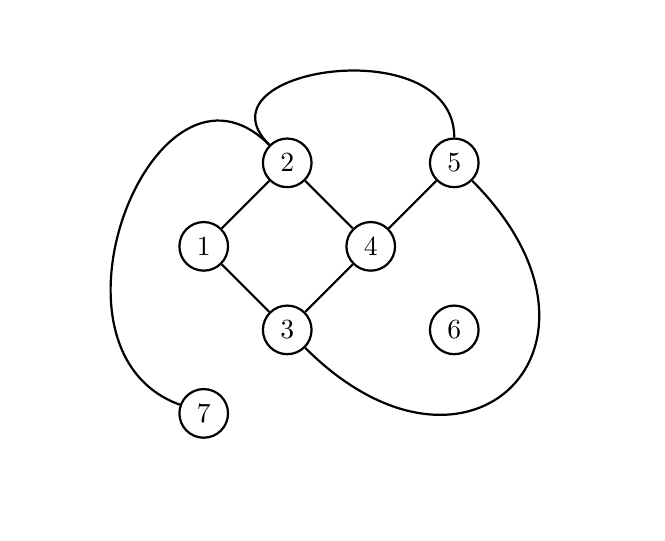
\begin{tikzpicture}[node distance={15mm}, thick, main/.style = {draw, circle}] 
\node[main] (1) {$1$}; 
\node[main] (2) [above right of=1] {$2$}; 
\node[main] (3) [below right of=1] {$3$}; 
\node[main] (4) [above right of=3] {$4$}; 
\node[main] (5) [above right of=4] {$5$}; 
\node[main] (6) [below right of=4] {$6$}; 
\node[main] (7) [below left of=3] {$7$}; 
\draw (1) -- (2); 
\draw (1) -- (3); 
\draw (2) to [out=135,in=90,looseness=1.5] (5); 
\draw (2) -- (4); 
\draw (3) -- (4); 
\draw (5) -- (4); 
\draw (5) to [out=315, in=315, looseness=2.5] (3); 
\draw (2) to [out=135, in=160, looseness=1.5] (7); 
\end{tikzpicture} 
\caption{Network $(a)$}
\end{minipage}
\hfill\begin{minipage}{.5\textwidth}\centering
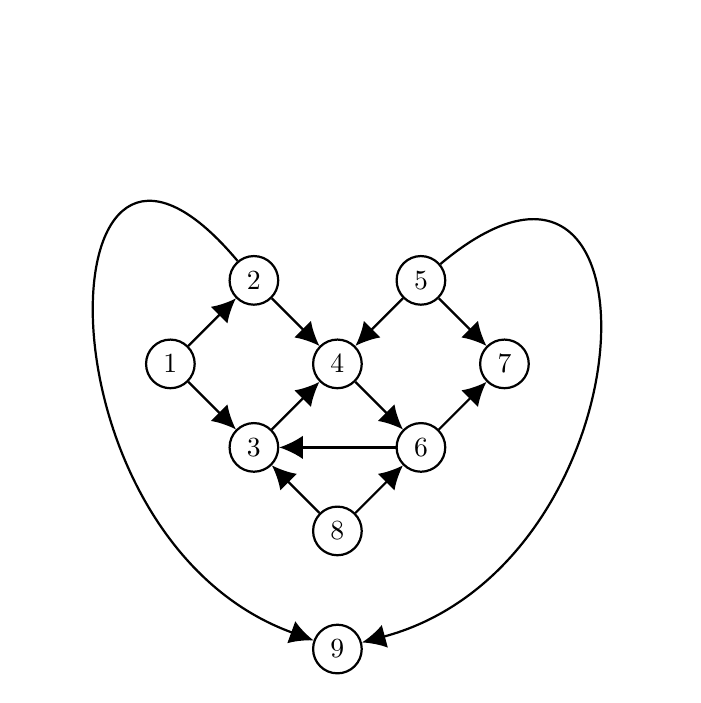
\begin{tikzpicture}[node distance={15mm}, thick, main/.style = {draw, circle}] 
\node[main] (1) {$1$}; 
\node[main] (2) [above right of=1] {$2$}; 
\node[main] (3) [below right of=1] {$3$}; 
\node[main] (4) [above right of=3] {$4$}; 
\node[main] (5) [above right of=4] {$5$}; 
\node[main] (6) [below right of=4] {$6$};
\node[main] (7) [below right of=5] {$7$}; 
\node[main] (8) [below right of=3] {$8$}; 
\node[main] (9) [below of=8] {$9$}; 
\draw[->] (1) -- (2); 
\draw[->] (1) -- (3); 
\draw[->] (3) -- (4); 
\draw[->] (4) -- (6); 
\draw[->] (6) -- (3); 
\draw[->] (2) to [out=130,in=160,looseness=2] (9);
\draw[->] (5) to [out=40,in=15,looseness=2] (9);
\draw[->] (2) -- (4); 
\draw[->] (8) -- (3); 
\draw[->] (8) -- (6); 
\draw[->] (6) -- (7); 
\draw[->] (5) -- (7); 
\draw[->] (5) -- (4); 
\end{tikzpicture} 
\caption{Network $(b)$}
\end{minipage}

\end{figure}


\noindent
\begin{enumerate}
	\item The corresponding adjacency matrices.
\item The corresponding link lists.
\item Determine the average clustering coefficient of Network $(a)$.
\item If you switch the labels of nodes 1 and 2 in Network $(a)$, how does that move change the adjacency matrix? \item And the link list?
\item What kind of information can you not infer from the link list representation of the network that you can infer from the adjacency matrix?
\item In the $(a)$ network, how many paths (with possible repetition of nodes and links) of length 4 exist starting from node 1 and ending at node 3? And in $(b)$?
\end{enumerate}



%%%%%%%%%%%%%%%%%%%%
\item \textit{Understanding Erdős-Rényi Networks}
%%%%%%%%%%%%%%%%%%%%

Consider an Erdős-Rényi network with $N = 3,000$ nodes, connected to each other with probability $p = 10^{–2}$.
\begin{enumerate}
    \item What is the expected number of links, 〈$L$〉?
\item In which regime is the network?
\item Calculate the probability $p_C$ so that the network is at the critical point.
\item Given the new linking probability $p = 10^{–3}$, calculate the number of nodes $N^{C.r}$ so that the network has only one component.
\item For the network in (d), calculate the average degree 〈$k^{Cr}$〉 and the average distance between two randomly chosen nodes 〈$d$〉.
\item Calculate the degree distribution $p_k$ of this network (approximate with a Poisson degree distribution).

\end{enumerate}

%%%%%%%%%%%%%%%%%%%%
\item \textit{Snobbish Networks}
%%%%%%%%%%%%%%%%%%%%

Consider a network of $N$ red and $N$ blue nodes. The probability that there is a link between nodes of identical color is $p$ and the probability that there is a link between nodes of different color is $q$. A network is snobbish if $p > q$, capturing a tendency to connect to nodes of the same color. For $q = 0$ the network has at least two components, containing nodes with the same color.

\begin{enumerate}
    \item Calculate the average degree of the ``blue" sub-network made of only blue nodes, and the average degree in the full network.
\item Determine the minimal $p$ and $q$ required to have, with high probability, just one component.
\item Show that for large $N$ even very snobbish networks ($p>>q$) display the small-world property.
\end{enumerate}


%%%%%%%%%%%%%%%%%%%%
\item \textit{Generating Erdős-Rényi Networks (coding question)}
%%%%%%%%%%%%%%%%%%%%

Relying on the G(N, p) model, generate with a computer three networks with $N = 300$ nodes and average degrees:
\begin{enumerate}
    \item 〈$k$〉 = 0.5
    \item 〈$k$〉 = 2  
    \item 〈$k$〉 = 10 
    \item Visualize these networks.
\end{enumerate}




%%%%%%%%%%%%%%%%%%%%
\item \textit{Calculating Network Metrics (coding question)}
%%%%%%%%%%%%%%%%%%%%

Using \href{https://networkx.org/documentation/stable/reference/index.html}{\textit{networkx}} library in \href{https://docs.python.org/3/}{\textit{python}} and the graph network data from \href{https://zenodo.org/record/1411479#.YzsonuzMJ6Q}{\textbf{Star Wars Episode IV Social Network}}, 

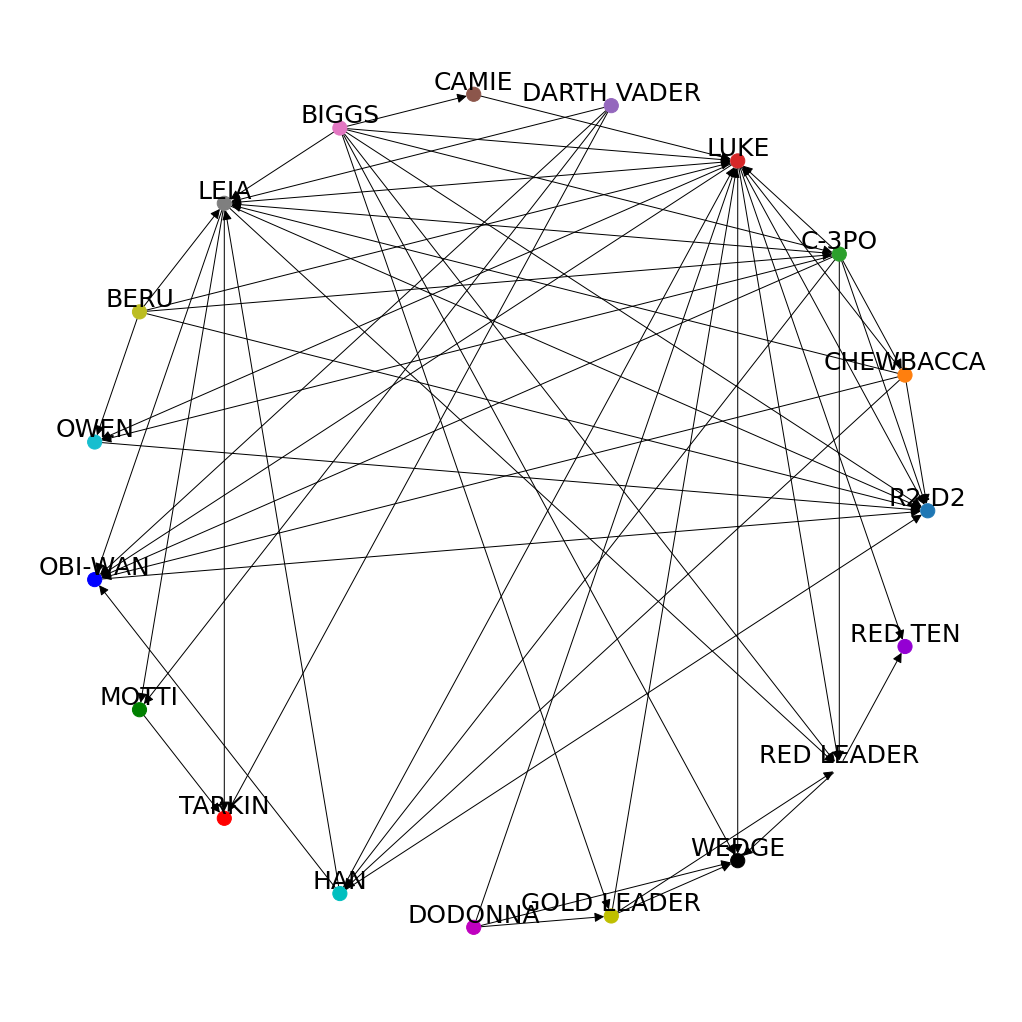
\includegraphics[height=9cm]{starwars_network.png}
\begin{enumerate}
    \item Find the following network metrics and compare them to a randomly generated network of the same number of nodes.
    \begin{enumerate}
        \item Average Degree Distribution
        \item Clustering Coefficient
    \end{enumerate}
    \item Summarize your observation from the metrics of both the networks.
    \item Explain in your own words what the difference in the metrics of the two networks say about the networks. (Imp Note: Make sure to provide an explanation for each metric listed above.)
    \item Plot Degree Distribution using \href{https://matplotlib.org/3.5.1/api/_as_gen/matplotlib.pyplot.html}{\textit{matplotlib-pyplot}}
    \item Write in your own words any inference that can be made from the plot.
\end{enumerate}



\end{enumerate}

\end{document}

% \documentclass{minimal}
% \usepackage{tikz}
% \usetikzlibrary{arrows}
% \begin{document}
% \newcounter{tmp}
% \begin{tikzpicture}
% \foreach \s in {latex,latex',stealth,triangle 90,triangle 45,angle 90, angle 60} {
%     \stepcounter{tmp}
%     \begin{scope}[yshift=-\thetmp cm]
%         \node[anchor=west] (0,0) {\texttt{\s}};     
%         \draw[arrows={\s-\s}] (3,0) --++ (1,0);
%     \end{scope}
% }
% \end{tikzpicture}
% \end{document}